\section{Task 2}
\label{sec:task2}

\subsection{Overview}
\label{subsec:desc2}

The second scenario tackles another multi-agent coordination task, colouring the 
robots according to a certain criterion in space. 
The environment, as well as the assumptions, are the same described in Chapter 
\ref{chap:experiments} and in Section \ref{subsec:desc1}.
%FIXME

The only difference lies in the goal to be achieved by the robots: assuming that 
the agents are divided into groups, their purpose is to colour themselves, by 
turning on their top \gls{rgb} \gls{led}, depending on their group membership.

Initially, for the sake of simplicity, we decided to divide the robots into two 
groups. In particular, in case of an even number of agents, the robots in the first 
half of the row belong to the first group and the remaining to the second, while in 
the case of an odd number robots, the agent located in the central position is 
assigned to the first set.

As for the previous task, the problem can be solved performing imitation 
learning, but the role of communication is fundamental. In fact, what makes the 
difference are not the distances perceived by the robot sensors but the messages 
exchanged between the agents, which are they only mean to determine their 
order. 

In this scenario, the two ``dead'' robots play an important role: they always 
communicate a message that indicates that they are the only two agents that 
receive communication just from one side.

Each agent can still update its state by performing actions — in this case not 
moving along the x-axis but colouring the top \gls{led} in red or blue — based on 
the observations received from the environment — the messages received from 
neighbours. 

Then, by following the example of an expert, we train an end-to-end \gls{nn} 
that takes as input the communication — transmitted by the nearest neighbours in 
the previous timestep — and produces the colour of the robot together with the 
message to be sent.

\subsection{Controllers}
\label{subsec:task2controllers}

\subsubsection{Expert controller}
\label{subsubsec:omniscient2}

As disclosed in Section \ref{subsec:controllersmodel}, the first element involved in 
an imitation learning problem is the omniscient controller, also called expert, 
which is able to perceive the environment and the observations of all the agents, 
obtaining a global knowledge of the state of the system. In this way it can use all 
the information to decide the best action to perform for each agent.

In this scenario, the omniscient controller, based on the current poses of each 
robot, is able to determine the order of the agents and turn on their top \gls{led}  
in one time step.

Unfortunately, neither this kind of problem can be solved using an expert since is 
not realistic nor feasible in a real environment.

\subsubsection{Manual controller}
\label{subsubsec:manual2}

The second controller we implemented is the manual one, whose main 
purpose is to draw conclusions about the quality of the learned controller.

The main difference between this and the previous controller is that, the manual 
one can be considered a local controller, that only has a partial knowledge of the 
environment since it knows only the state of the current agent and its 
observations.

For this scenario, the robots observation, in particular the sensor readings, do not 
provide useful information about the order of the agents, therefore they are not 
considered to accomplish this task.
On the other hand, if an omniscient controller is not employed, it is impossible to 
solve the problem without using communication, since it is the only way for the 
agents to understand they ordering.

Thus, by initially making all robots transmit the same value, i.e. $0$, we are able 
to establish which are the first and the last robots in the row, or those that do not 
receive any communication respectively from back and front. 
These two agents can at this point start the actual communication by transmitting 
the value they received increased by $1$, that is $1$. 
The following robots will in turn transmit the value they have received increased 
by one. Since the messages received by each of them are two, the agents will in a 
sense, learn to count in order to understand which is the correct value to 
transmit.

The protocol used to decide the communication and the colour, which also 
depends on the amount of robots $N$, or if there are even or odd numbers, is 
shown in Listing \ref{lst:manualtask2}. The colour of each agent in the initial 
configuration is randomly chosen between the two possible colours, red and blue.

\begin{python}
c_left, c_right = get_received_communication(state)

if N % 2 == 1:  # if the number of robots is odd

	# Case 1: no communication received from left
	if c_left == 0:
		if c_right > N // 2:
			# the agent is in the first half of the row, so its colour is blue
			message = c_right - 1
			colour = 1
		elif c_right == N // 2:
			# the agent is the central one, so its colour is blue
			message = c_right + 1
			colour = 1
		else:
			# the agent is in the second half of the row, so its colour is red
			message = c_right + 1
			colour = 0
			
	# Case 2: no communication received from right
	elif c_right == 0:
		if c_left > N // 2:
			# the agent is in the second half of the row, so its colour is red
			message = c_left - 1
			colour = 0
		elif c_left == N // 2:
			# the agent is the central one, so its colour is blue
			message = c_left + 1
			colour = 1
		else:
			# the agent is in the first half of the row, so its colour is blue
			message = c_left+ 1
			colour = 1
			
	# Case 3: communication received from both sides
	else:
		if c_left > c_right:
			# the agent is in the second half of the row, so its colour is red
			message = c_right + 1
			colour = 0
		else:
			# the agent is in the first half of the row, so its colour is blue
			message = c_left + 1
			colour = 1


elif self.N % 2 == 0:  # if the number of robots is even

	# Case 1: no communication received from left
	if c_left == 0:
		if c_right > N // 2:
			# the agent is in the first half of the row, so its colour is blue
			# the situation is ambiguous the message to transmit could be c_right or 
			# even c_right - 1
			message = c_right
			colour = 1
		else:
			# the agent is in the second half of the row, so its colour is red
			message = c_right + 1
			colour = 0
	
	# Case 2: no communication received from right
	elif c_right == 0:
		if c_left < N // 2:
			# the agent is in the first half of the row, so its colour is blue
			message = c_left + 1
			colour = 1
		else:
			# the agent is in the second half of the row, so its colour is red
			# the situation is ambiguous the message to transmit could be c_left or 
			# even c_left - 1
			message = c_left
			colour = 0
	
	# Case 3: communication received from both sides
	else:
		if c_left > c_right:
			# the agent is in the second half of the row, so its colour is red
			message = c_right + 1
			colour = 0
		elif c_left < c_right:
			# the agent is in the first half of the row, so its colour is blue
			message = c_left + 1
			colour = 1
		else:
			# the agent is in the second half of the row, so its colour is red
			message = c_left
			colour = 0
\end{python}

\begin{lstlisting}[frame=none,caption=Protocol used from the manual controller 
to decide for each robot the message to transmit and the colour., 
label=lst:manualtask2]
\end{lstlisting}


\subsection{Communication approach}
\label{subsec:task2comm}

\subsubsection{Model training}
\label{subsubsec:learnedcomm2}
For this purpose, it is possible to use the same network used in the previous task, 
that means the one implemented for the distributed approach with 
communication, but this time ignoring the sensors readings.
Thus, using the same data collected before we build a model that at each time 
step takes as input for each robot only the message received in the previous time 
step, communicated by the nearest agents (on the left and on the right), and 
produces as output an array of 2 floats, the first one is the probability of the agent 
top \gls{led} to be blue and the second is the communication, i.e. the message to 
be transmitted by the robot.

The structure of the communication network is shown in Figure 
\ref{fig:commnet2}, and as before it is composed by two nested 
modules: 
\begin{figure}[!htb]
	\centering
	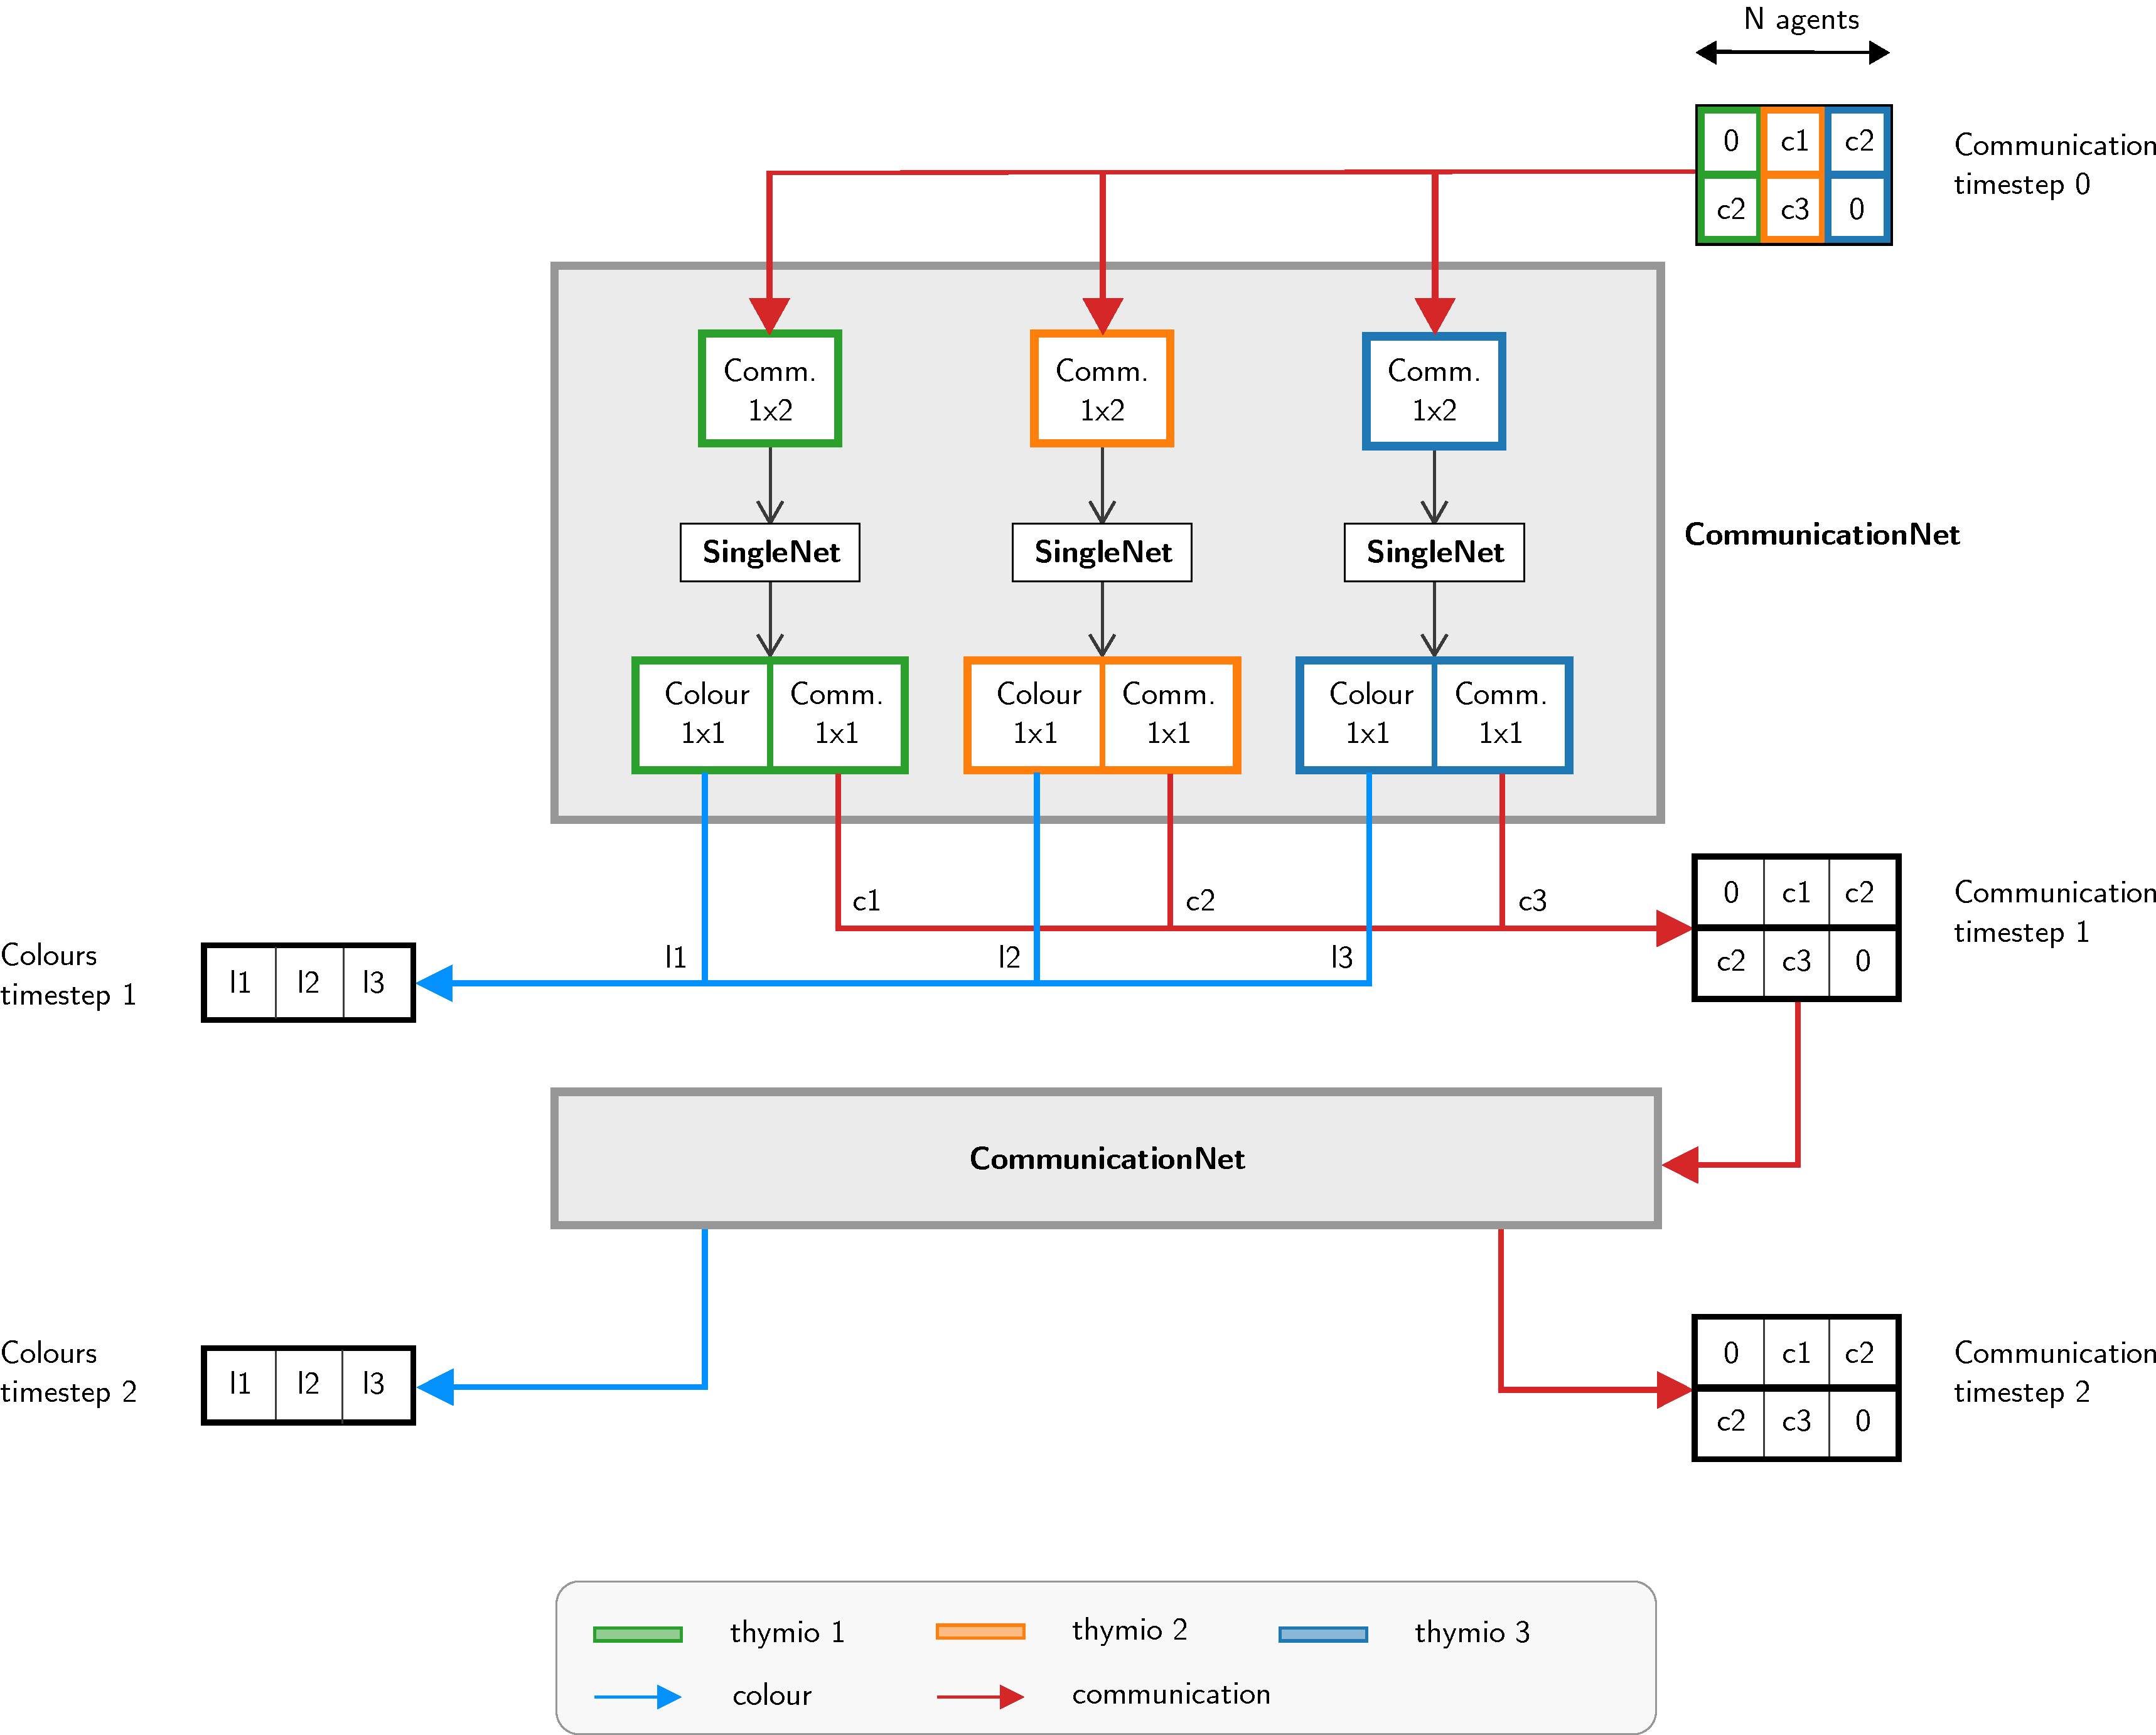
\includegraphics[width=\textwidth]{contents/images/commnettask2}
	\caption[Communication network of the second task.]{Visualisation of the 
		forward pass of the communication network with three agents and a 
		sequence 
		composed by two time steps.}
	\label{fig:commnet2}
\end{figure}
in the outer-level operates the \texttt{CommNet} that handle the 
sensing of all the agents, while in the inner-level the \texttt{SingleNet} that 
works on the communication received by a single agent in a certain time 
step, producing as output the colour and the communication to transmit. 
The \texttt{SingleNet}, displayed in Figure \ref{fig:singlenetcomm2}, is composed 
by three linear layers of size $\langle \mathtt{input\_size}, 10\rangle$,  $\langle 
10, 10\rangle$ and $\langle 10, 2\rangle$, where \texttt{input\_size} 
corresponds to the two communication values received, one from the left and one 
from the right.
\begin{figure}[!htb]
	\centering
	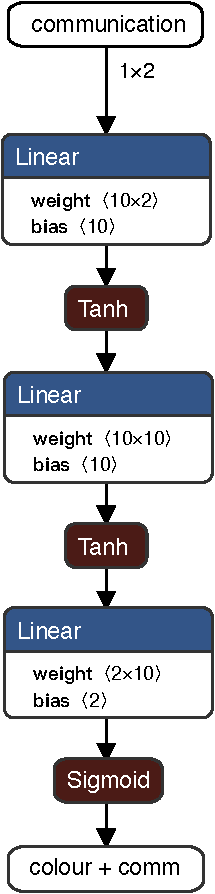
\includegraphics[width=.15\textwidth]{contents/images/task2allcomm}
	\caption[Network architectures for the communication approach.]{Visualisation 
	of the network architecture chosen for the 
		communication approach.}
	\label{fig:singlenetcomm2}
\end{figure}

The activation functions used for this purpose are two and are shown in 
Figure \ref{fig:activation}.
To the first and second layer is applied a Tanh non-linear activation function, 
while a sigmoid to the output, in order to normalise it in the range $[0, 1]$.
\begin{figure}[!htb]
	\begin{center}
		\begin{subfigure}[h]{0.495\textwidth}
			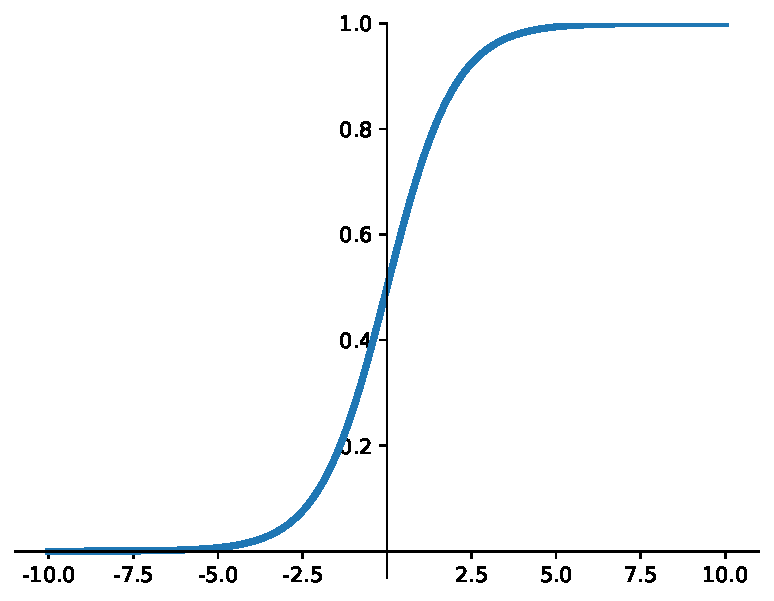
\includegraphics[width=\textwidth]{contents/images/sigmoid2}
			\caption{Tanh activation function}
		\end{subfigure}
		\hfill
		\begin{subfigure}[h]{0.495\textwidth}
			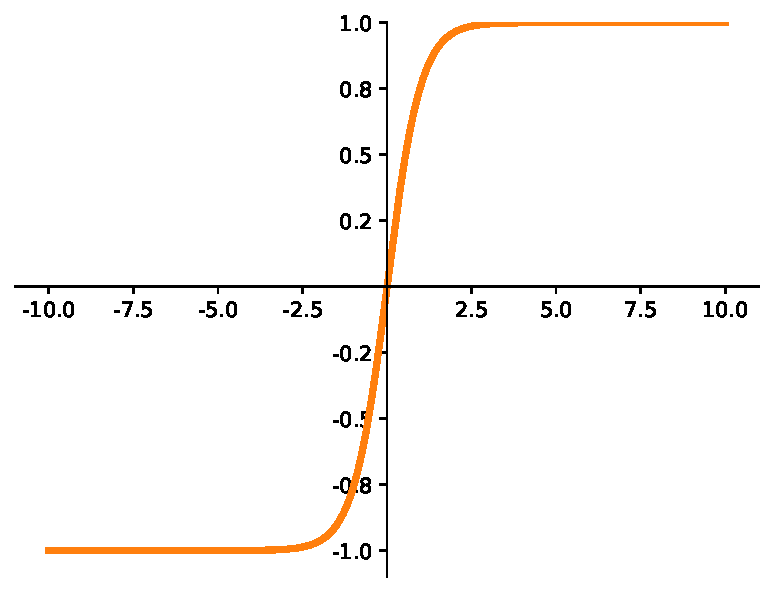
\includegraphics[width=\textwidth]{contents/images/tanh2}
			\caption{Sigmoid activation function.}
		\end{subfigure}
	\end{center}
	\caption{Trend of the activation functions applied as non-linear activations.}
	\label{fig:activation}
\end{figure}

As before, we use Adam optimiser but with a smaller learning rate, $0.001$. 
We split the dataset in mini-batches of size $10$ and then we train the models for 
$100$ epochs. 

In order to decide the metric to evaluate the goodness of the prediction it is 
necessary to analyse the output of the network. As we said, the model returns, in 
addition to the communication, the colour that is actually the probability of the 
agent top \gls{led} to be blue. This means that, when the network produces a 0, 
the probability that the \gls{led} is blue is equal to 0, i.e. is red, in the same way 1 
means that instead this will be blue. In this way, we define a simple policy function 
that returns the colour blue when the probability is between 0.5 and 1, and red 
otherwise, or when the probability is less than 0.5.
For this reason, instead of using the \gls{mse} loss function, as this is a binary 
classification problem we choose the \gls{bce}, defined as follows:
\begin{Equation}[H]
	\centering
	\begin{equation}
	\mathtt{BCE} = -\frac{1}{n} \sum_{i=1}^n \log(p(y_i)) + (1-y_i) \cdot \log(1 - 
	p(y_i))
	\end{equation}
	\caption{Binary Cross Entropy (\gls{bce}) loss function.}
	\label{eq:bce}
\end{Equation}
where $y$ is the target (1 for blue and 0 for red), $p(y)$ is the predicted 
probability of the \gls{led} of being blue for all $N$.
This loss function should return high values for bad predictions and low values for 
good ones.
It is important to remember that the communication is still learned in an 
unsupervised way.

\subsubsection{Experiments}
\label{subsubsec:expcomm2}

In this section we explore the experiments carried out using the communication 
approach, in particular, examining the behaviour of the control learned from 9 
networks based on different simulation runs that use a number of robots $N$ that 
can be fixed at $5$ or $8$ for the entire simulation, or even vary in the range $[5, 
10]$, and an \texttt{avg\_gap} that can be a fixed value in all the runs, chosen 
between $8$ or $20$, but also vary in the range $[5, 24]$. 
The objective of this set of experiments, summarised in Table 
\ref{tab:modelcommt2}, is to verify the robustness of the communication 
protocol and prove also the scalability of the network on the number of agents.
\begin{figure}[!htb]
	\centering
	\begin{tabular}{ccc}
		\toprule
		\textbf{Model} \quad & \textbf{\texttt{avg\_gap}} & \textbf{\texttt{N}}\\
		\midrule
		\texttt{net-v1}   &  $8$		 &	 $5$ \\
		\texttt{net-v2}   &  $20$		&	$5$ \\
		\texttt{net-v3}   &  variable   &    $5$\\
		\texttt{net-v4}   &  $8$		 &	  $8$ \\
		\texttt{net-v5}   & $20$   		&	 $8$ \\
		\texttt{net-v6}   &  variable	&	 $8$ \\
		\texttt{net-v7}   &  $ 8$		  &	 variable\\
		\texttt{net-v8}   &  $20$		 &	variable\\
		\texttt{net-v9}   &  variable	 &	variable\\
		\bottomrule
	\end{tabular}
	\captionof{table}[Experiments with variable agents and gaps 
	(communication).]{List of the experiments carried out using a variable number 
	of agents and of gap.}
	\label{tab:modelcommt2}
\end{figure}

First of all we start by showing in Figure \ref{fig:t2lossallt} an overview of the train 
and validation losses obtained for these models.
Then, we move on focusing our examination by inspecting the behaviour of the 
network trained on simulations with variable average gap, i.e \texttt{net-v3}, 
\texttt{net-v6} and \texttt{net-v9} and we summarise in Figure 
\ref{fig:commlossn5t2} the losses of 
\begin{figure}[!htb]
	\centering
	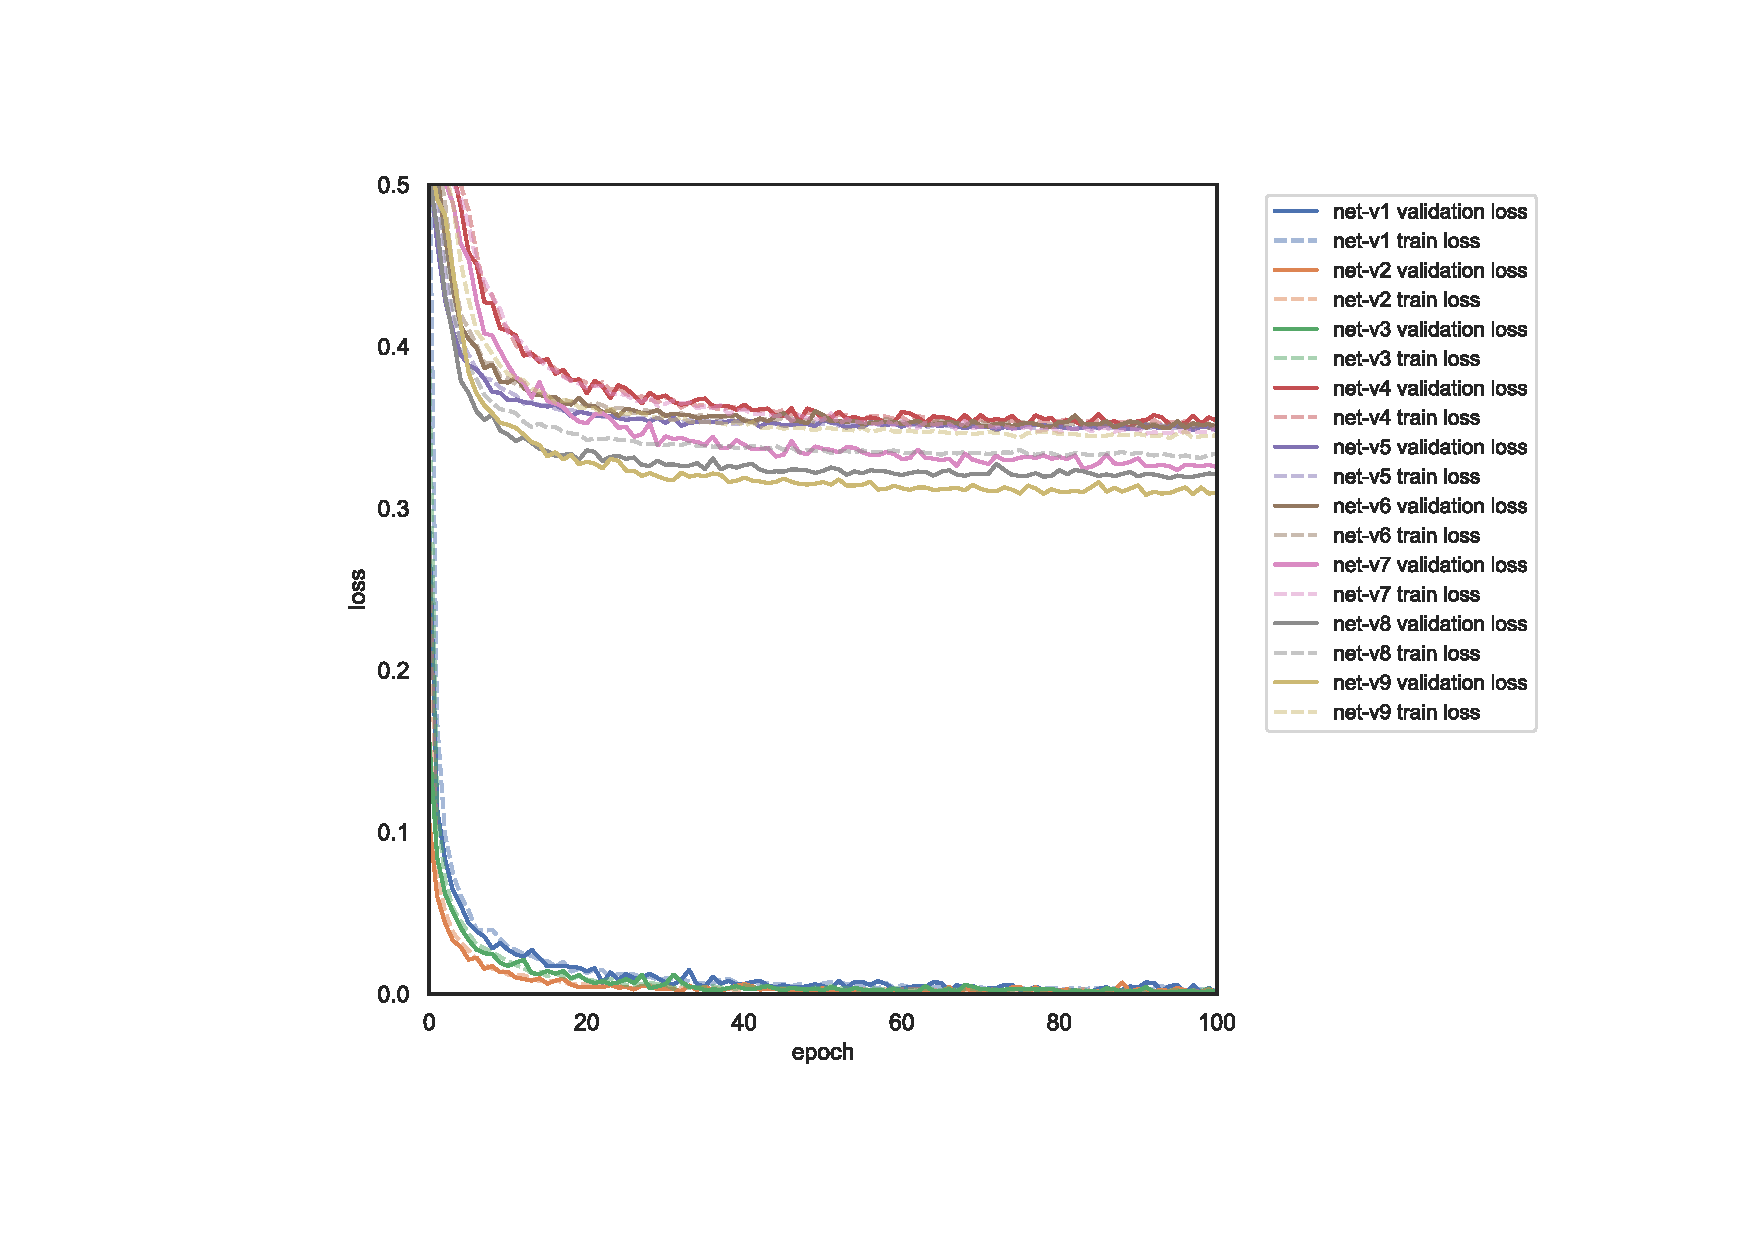
\includegraphics[width=.7\textwidth]{contents/images/task2/loss-communication-all@}%
	\caption[Comparison of losses of the second set of experiments.]{Comparison 
		of the losses of the models carried out using a variable number of agents and 
		of average gap.}
	\label{fig:t2lossallt}
\end{figure}

\noindent
these experiments in order to highlight the 
difference of performance using a gap that is first small, then large and finally 
variable, respectively represented by the blue, the orange and the green lines.
Clearly, in case of small gaps the network performs better, albeit slightly, as the 
agents are already close to the target.

\begin{figure}[!htb]
	\centering
	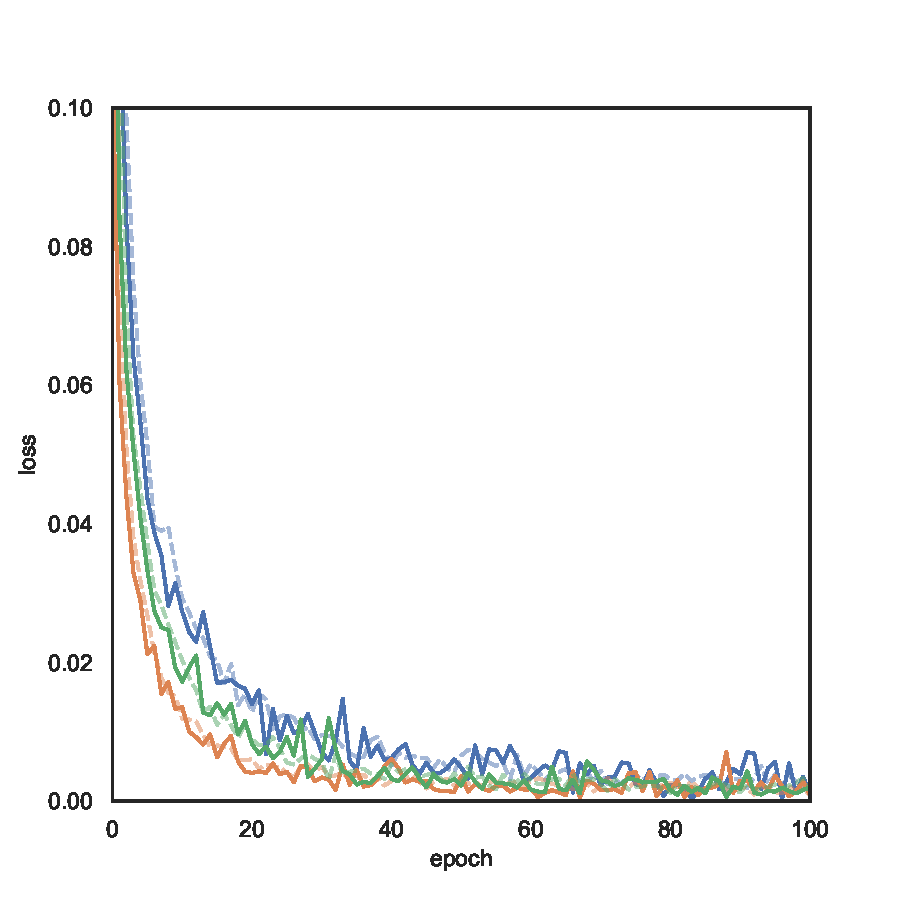
\includegraphics[width=.45\textwidth]{contents/images/task2/loss-communication-N5}
	\caption{Comparison of the losses of the models that use $5$ agents as the gap 
		varies.}
	\label{fig:commlossn5t2}
\end{figure}
	
We start the analysis by exploring the results of the experiments by showing in 
Figure \ref{fig:net-v3auc} the \gls{roc} curve of the model 
\cite[see][]{fawcett2006introduction}, a visualisation of the performance of our 
classification model, in terms of \gls{tpr} versus \gls{fpr}, at all classification 
thresholds.
In particular we use the \gls{auc} to evaluate the classifier: by measuring the 
\gls{2d} area under the ROC curve, from $[0, 0]$ to $[1, 1]$, the \gls{auc} is able 
to provide an aggregate measure of performance as the discrimination threshold 
varies.
We assume that a model whose predictions are 100\% correct has an \gls{auc} of 
1, as in this case.
\begin{figure}[!htb]
	\centering
	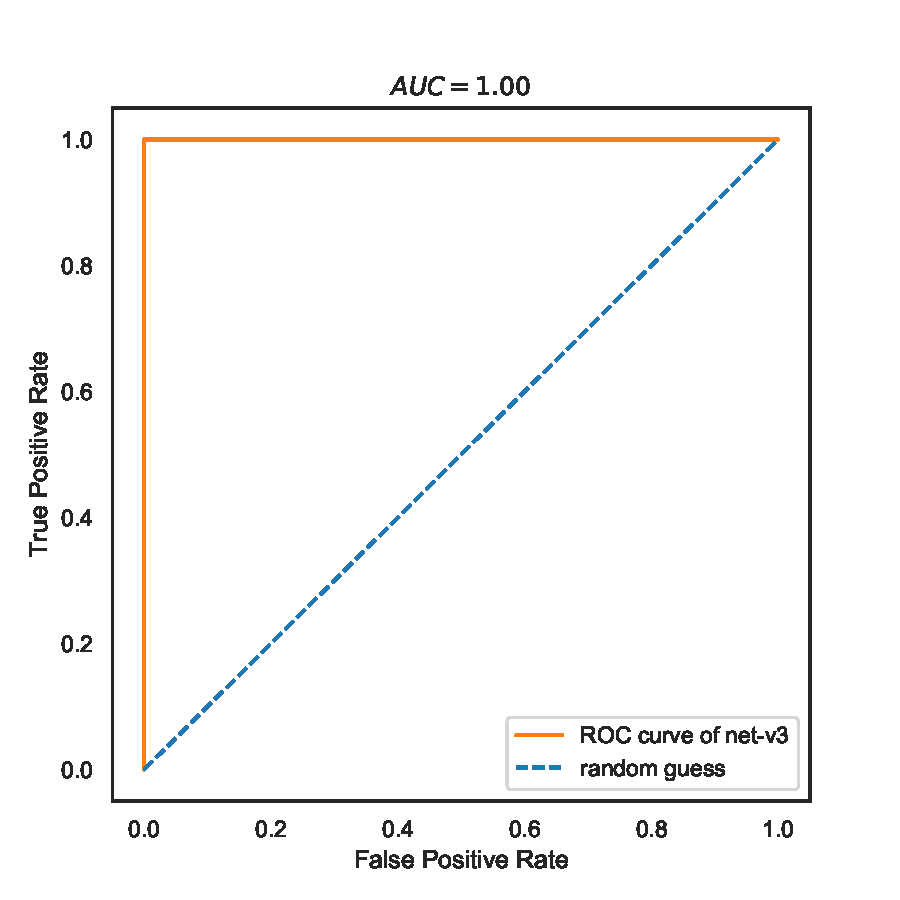
\includegraphics[width=.45\textwidth]{contents/images/net-v3/roc-net-v3(a)}%
	\caption[Evaluation of the \gls{roc} of \texttt{net-v3}.]{Visualisation of the 
		\gls{roc} curve of \texttt{net-v3}.}
	\label{fig:net-v3auc}
\end{figure}

%Moreover, we show another metric for evaluating our model, the accuracy, that 
%is the fraction of the number of correct predictions over the total number of 
%samples. In this case the value obtained is not very satisfactory, as we reach an 
%accuracy of only $66\%$.

Also for this task it is interesting to analyse the type of communication protocol 
inferred by the network, also comparing it with the one implemented by the 
manual controller. In Figure \ref{fig:net-v3commcolour} are shown, for a 
simulation run, first the messages transmitted by the agents over time, through a 
colour bar whose spectrum is included in the range [0, 1], i.e. the maximum and 
minimum value of communication transmitted, and then the colour assumed bt 
the robot in a certain time step, for both the manual and the learned controllers.
The extreme robots always transmit the same message using both controllers, 
while using the learned one, the central robots seems to transmit the same value, 
i.e. 1, but despite this they are able to achieve their goal in only two time steps, 
one less than with the manual. This behaviour cannot scale to a number of robot 
higher then $5$. For instance, in case of $5$ agents, in the first time step, 
\texttt{myt2} and \texttt{myt4} receive respectively the messages $(0, 1)$ and $(1, 
0)$, so they immediately know their position with respect to the central robot, 
which in turn knows its position since it receives $(1, 1)$. Then they communicate 
their message and in the following time step all the agents have coloured 
themselves in the right way, achieving the goal.
Consequently if the number of robots is greater, the central robots are not able to 
localise themselves. 
\begin{figure}[!htb]
	\begin{subfigure}[h]{\textwidth}
		\centering
		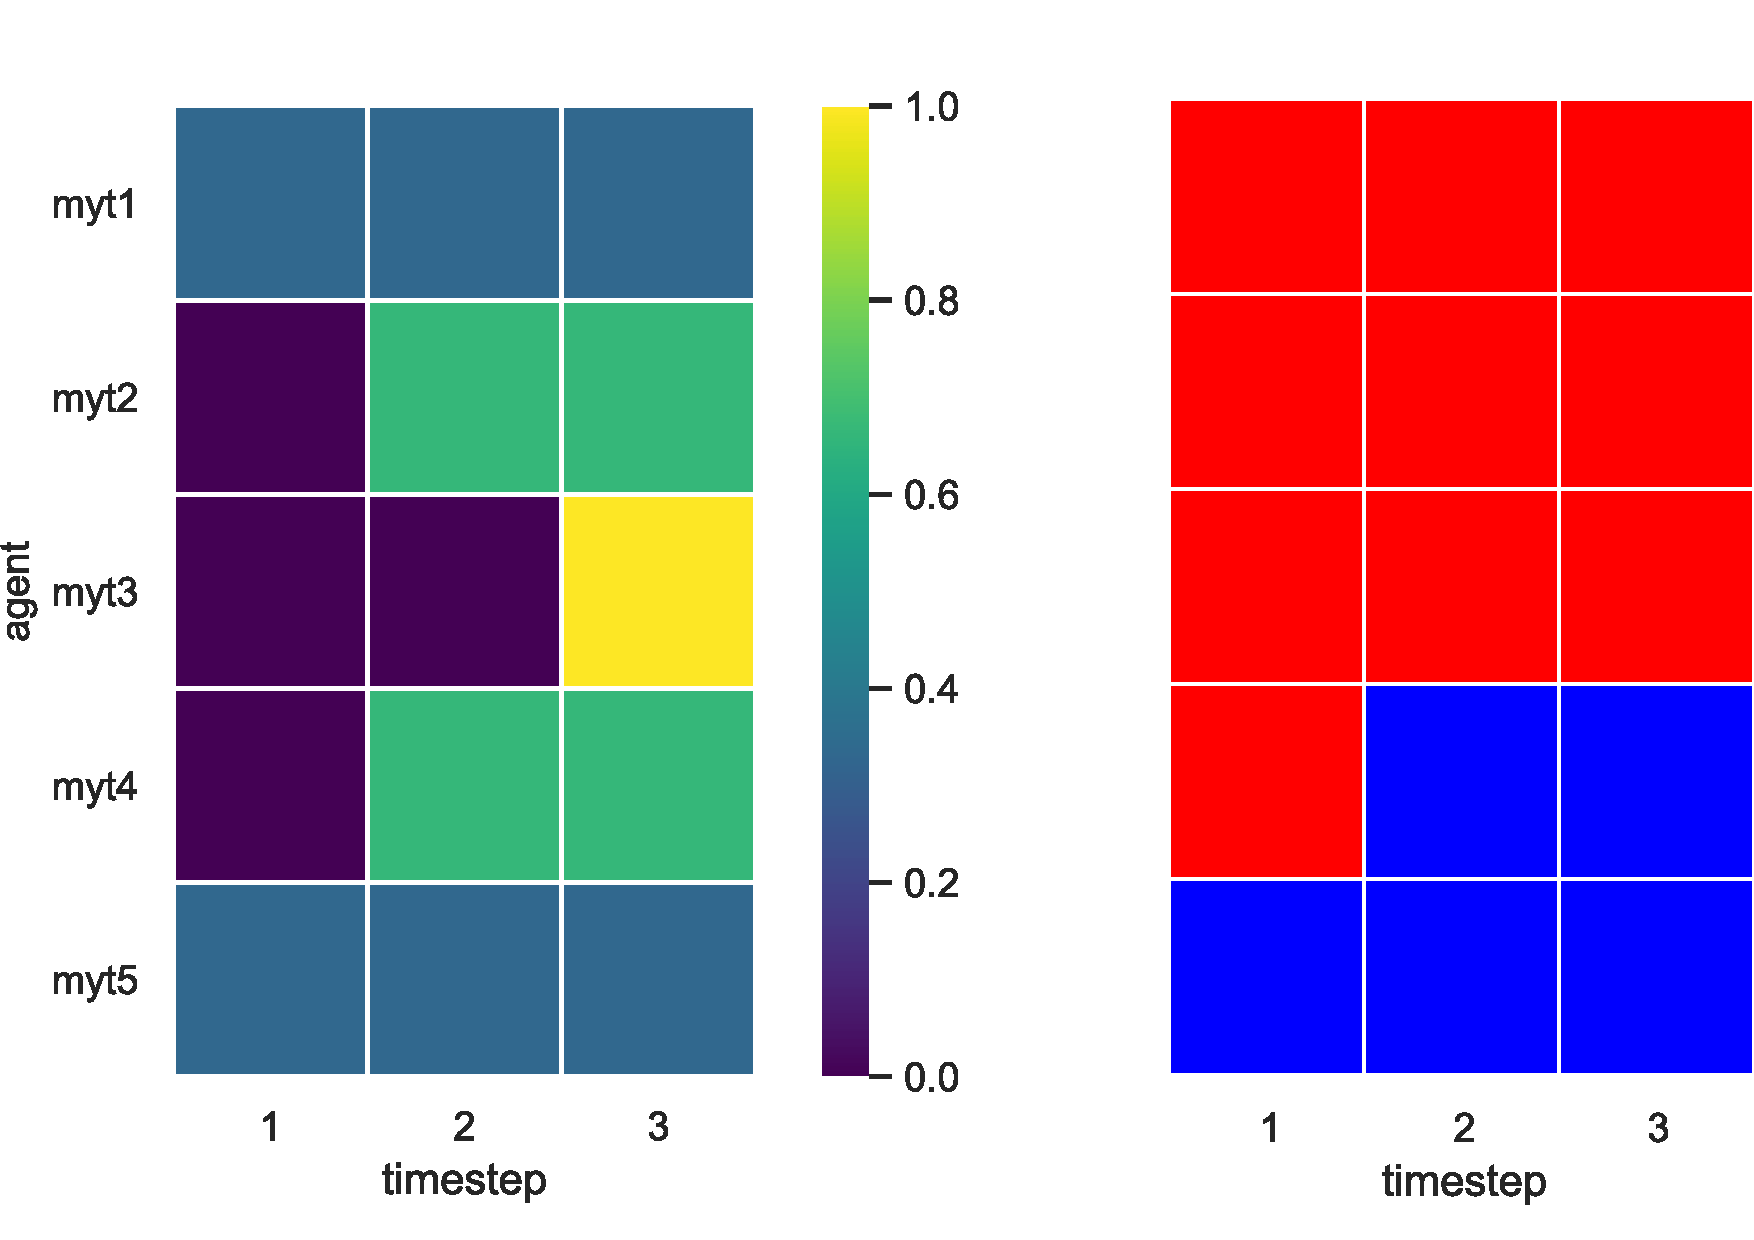
\includegraphics[width=.45\textwidth]{contents/images/net-v3/manual-0}
		\caption{Communication and colour decided using the manual controller.}
	\end{subfigure}
	\hspace*{\fill}%          % empty line absolutely necessary!
	\vspace*{8pt}%  
	\hspace*{\fill}%  
	\begin{subfigure}[h]{\textwidth}
		\centering			
		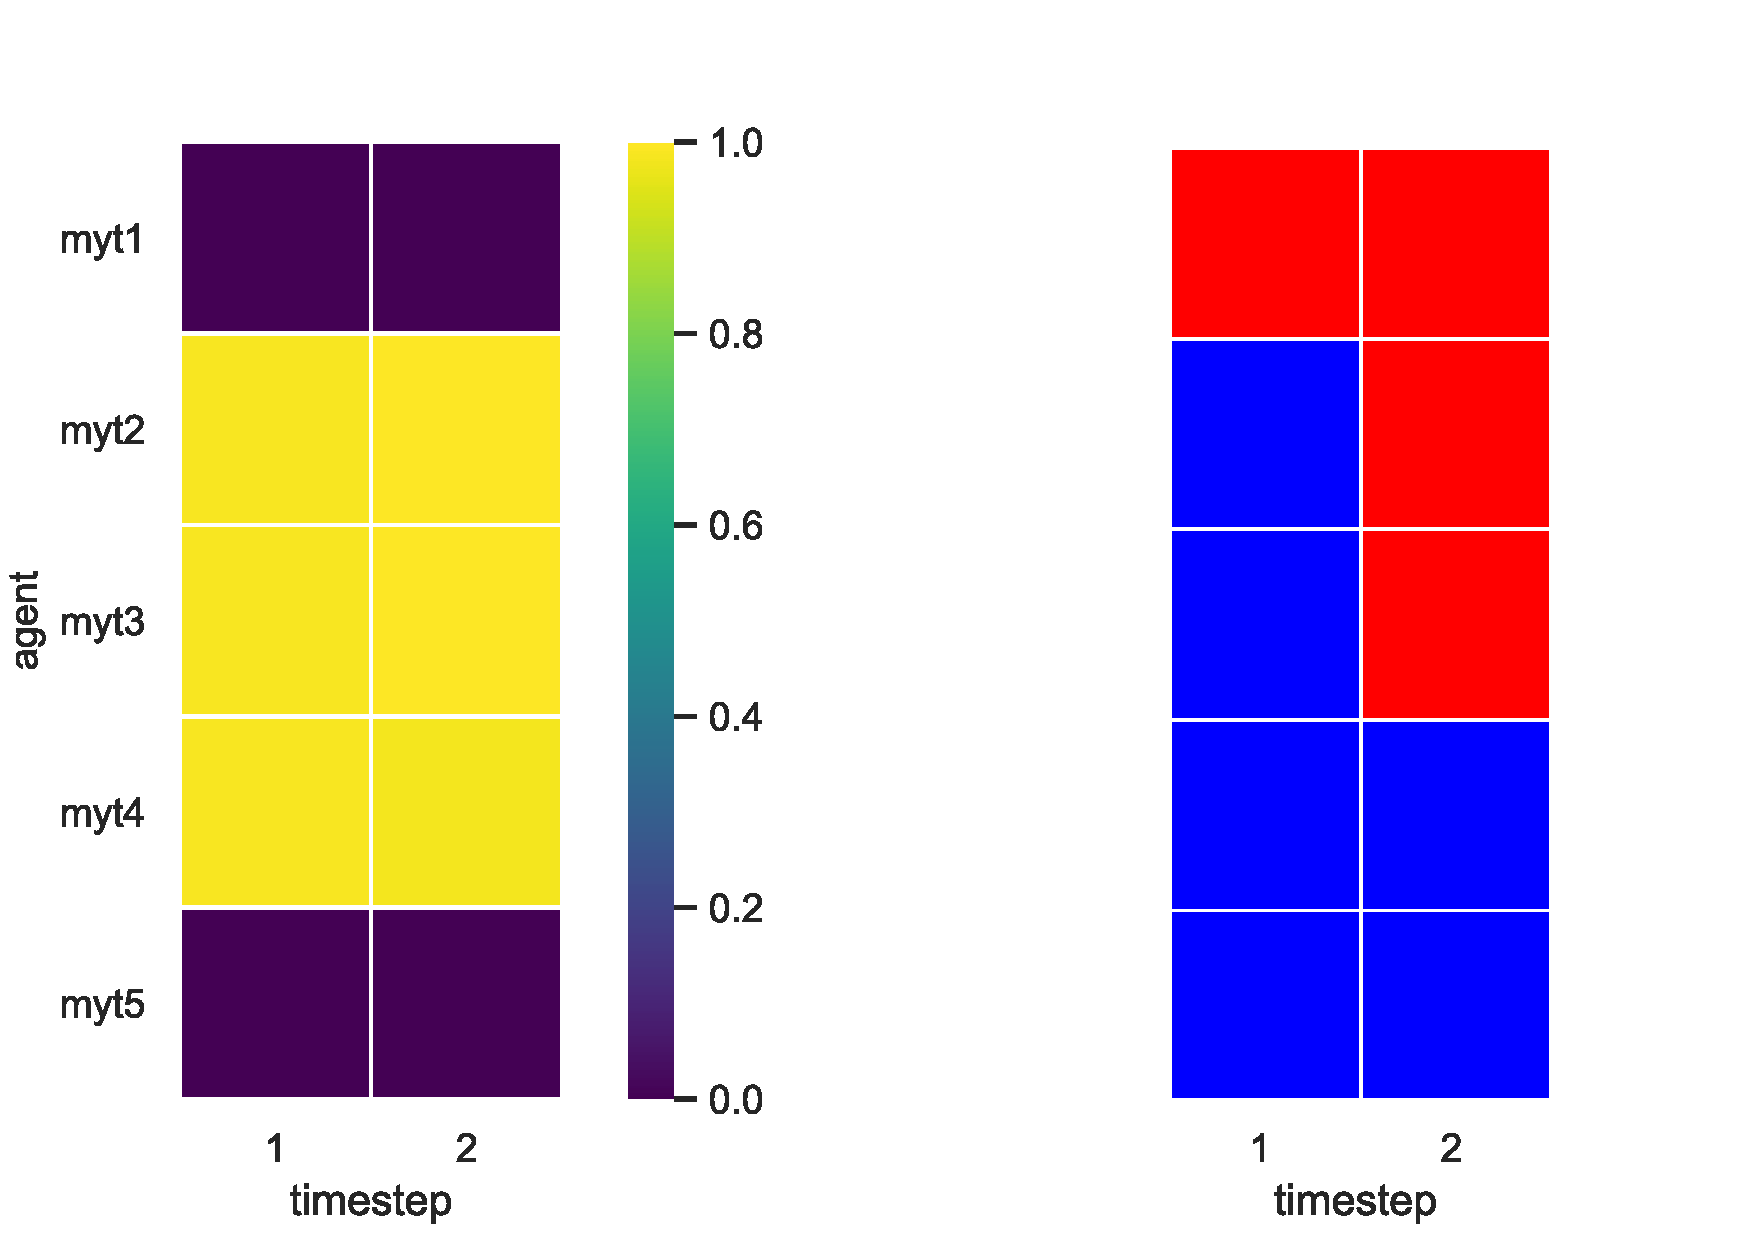
\includegraphics[width=.45\textwidth]{contents/images/net-v3/learned-0}
		\caption{Communication and colour decided using the learned controller.}
	\end{subfigure}
	\caption[Evaluation of the communication learned by 
	\texttt{net-v3}.]{Visualisation of the communication transmitted by each 
		robot over time and the colour decided by the controller learned from 
		\texttt{net-v3}.}	
	\label{fig:net-v3commcolour}
\end{figure}

In Figure \ref{fig:net-v3error} is presented a useful metric that measures the 
amount of wrong expected colours, on the y-axis, over time, averaged for all the 
robots among the simulation runs. In particular, at each time step we count the 
number of agents that have the wrong colour and divide it by the number of 
simulations.
The mean value is shown as well as the bands representing minus and plus the 
standard deviation.
On average, the amount of correct colours is higher for the manual controller 
than the learned one. 
\begin{figure}[!htb]
	\centering
	\includegraphics[width=.5\textwidth]{contents/images/net-v3/colours-errors-compressed}%
	\caption[Evaluation of \texttt{net-v3} amount of wrong expected 
	colours.]{Comparison of performance in terms of amount of wrong expected 
	colours obtained using the controller learned from \texttt{net-v3}.}
	\label{fig:net-v3error}
\end{figure}

Following are presented the results of the experiments performed using $8$ 
agents, in particular, in Figure \ref{fig:commlossn8t2} are summarised the 
performance in terms of train and validation losses, by varying the average gap, as 
before the blue, orange and green 
\begin{figure}[!htb]
	\centering
	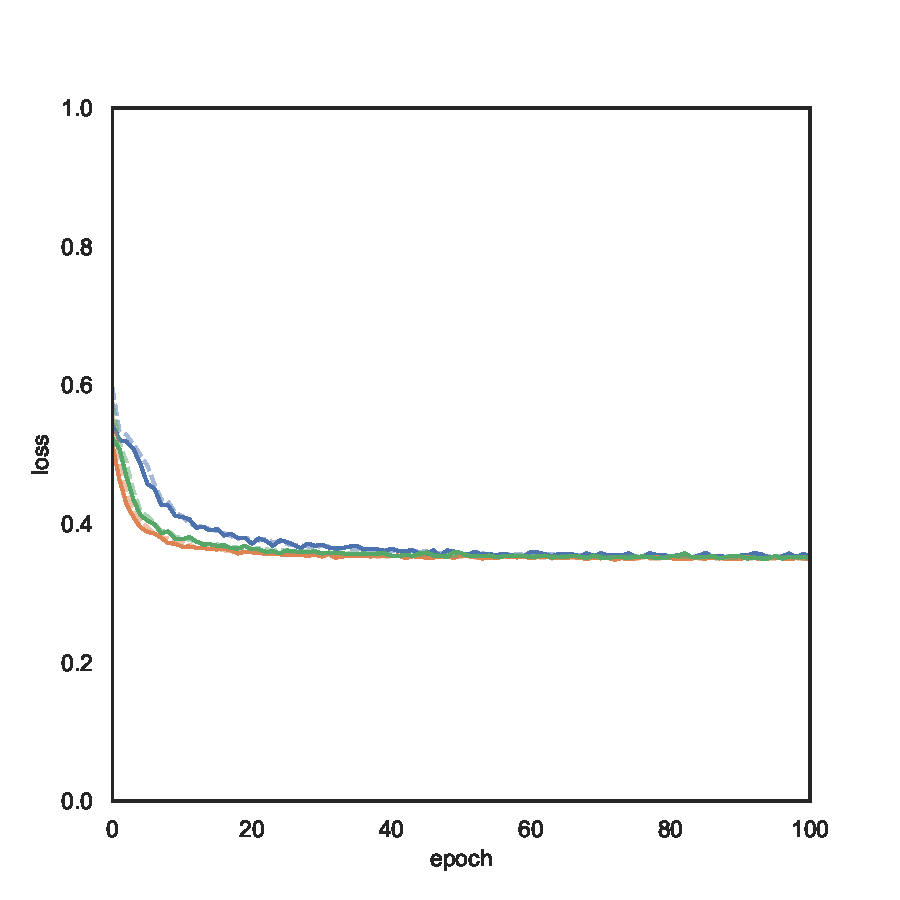
\includegraphics[width=.45\textwidth]{contents/images/task2/loss-communication-N8}
	\caption{Comparison of the losses of the models that use $8$ agents as the gap 
		varies.}
	\label{fig:commlossn8t2}
\end{figure}

\noindent
lines represent respectively gaps of $8$\gls{cm}, $20$\gls{cm} and variable. 
From a first observation we see that the losses are higher than before, this is 
because a higher number of agents reduce the performance of the models, since 
a higher number of time step is necessary to achieve te goal.

From the \gls{roc} curve of the model in Figure \ref{fig:net-v6auc} we observe 
that this time the \gls{auc} is decreased from 1 to 0.87 with respect to the 
previous model examined. 
%, while the accuracy is increased from $66\%$ up to $73\%$, 
\begin{figure}[!htb]
	\centering
	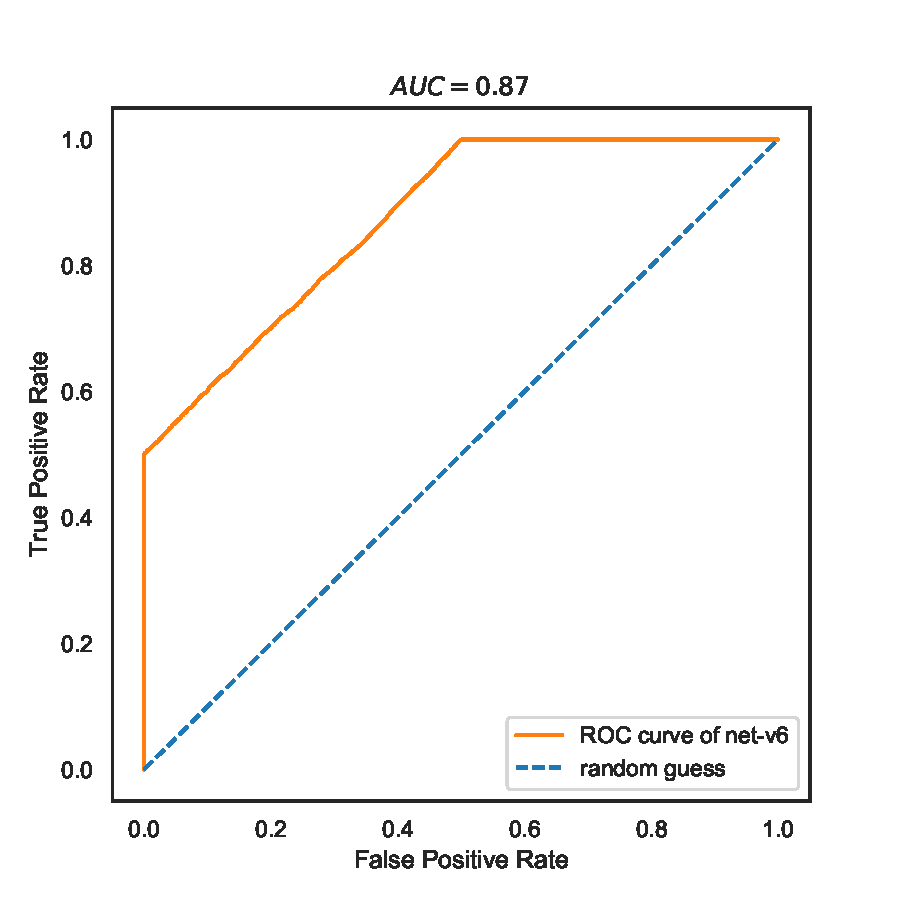
\includegraphics[width=.45\textwidth]{contents/images/net-v6/roc-net-v6(a)}%
	\caption[Evaluation of the \gls{roc} of \texttt{net-v6}.]{Visualisation of the 
		\gls{roc} curve of \texttt{net-v6} based on \gls{bce} Loss.}
	\label{fig:net-v6auc}
\end{figure}

\begin{figure}[!htb]
	\begin{subfigure}[h]{\textwidth}
		\centering
		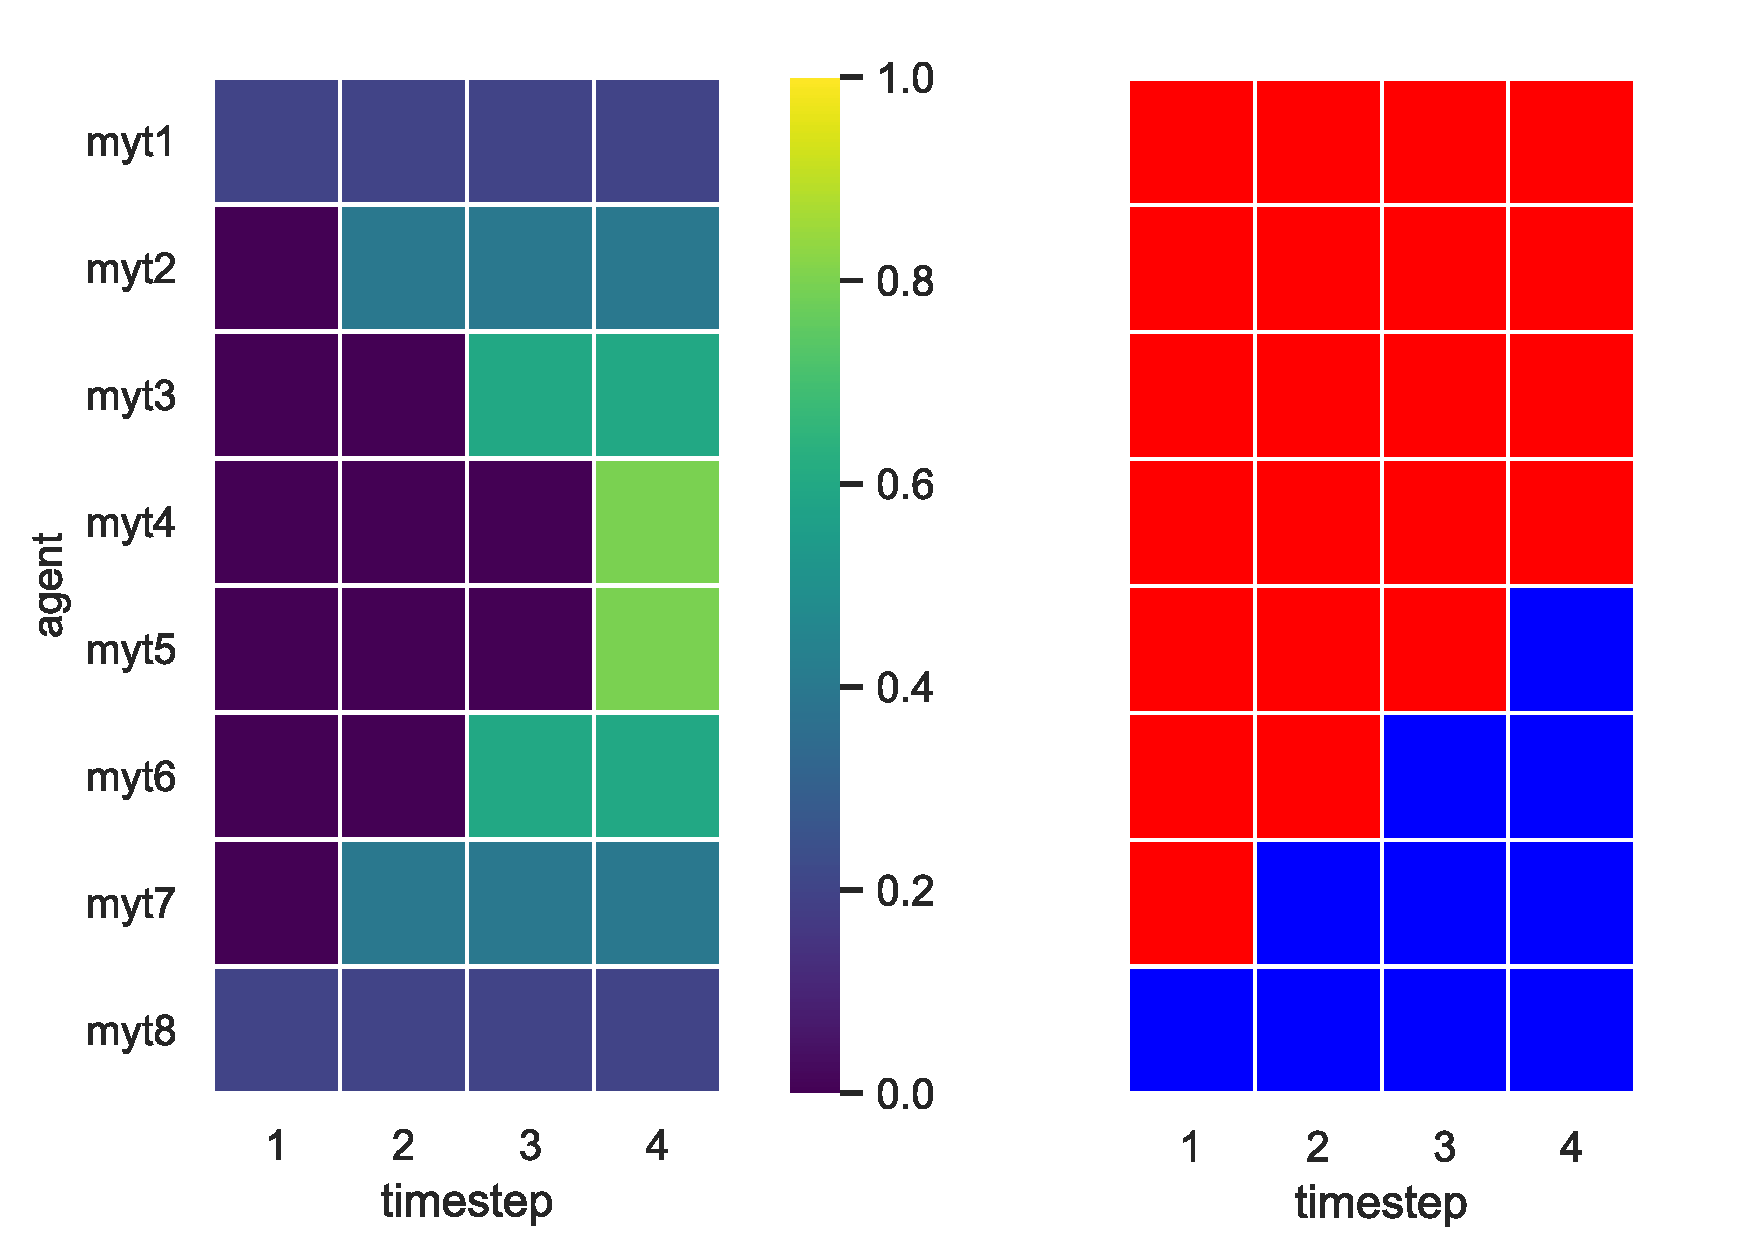
\includegraphics[width=.55\textwidth]{contents/images/net-v6/manual-0}
		\caption{Communication and colour decided using the manual controller.}
	\end{subfigure}
	\hspace*{\fill}%          % empty line absolutely necessary!
	\vspace*{8pt}%  
	\hspace*{\fill}%  
	\begin{subfigure}[h]{\textwidth}
		\centering			
		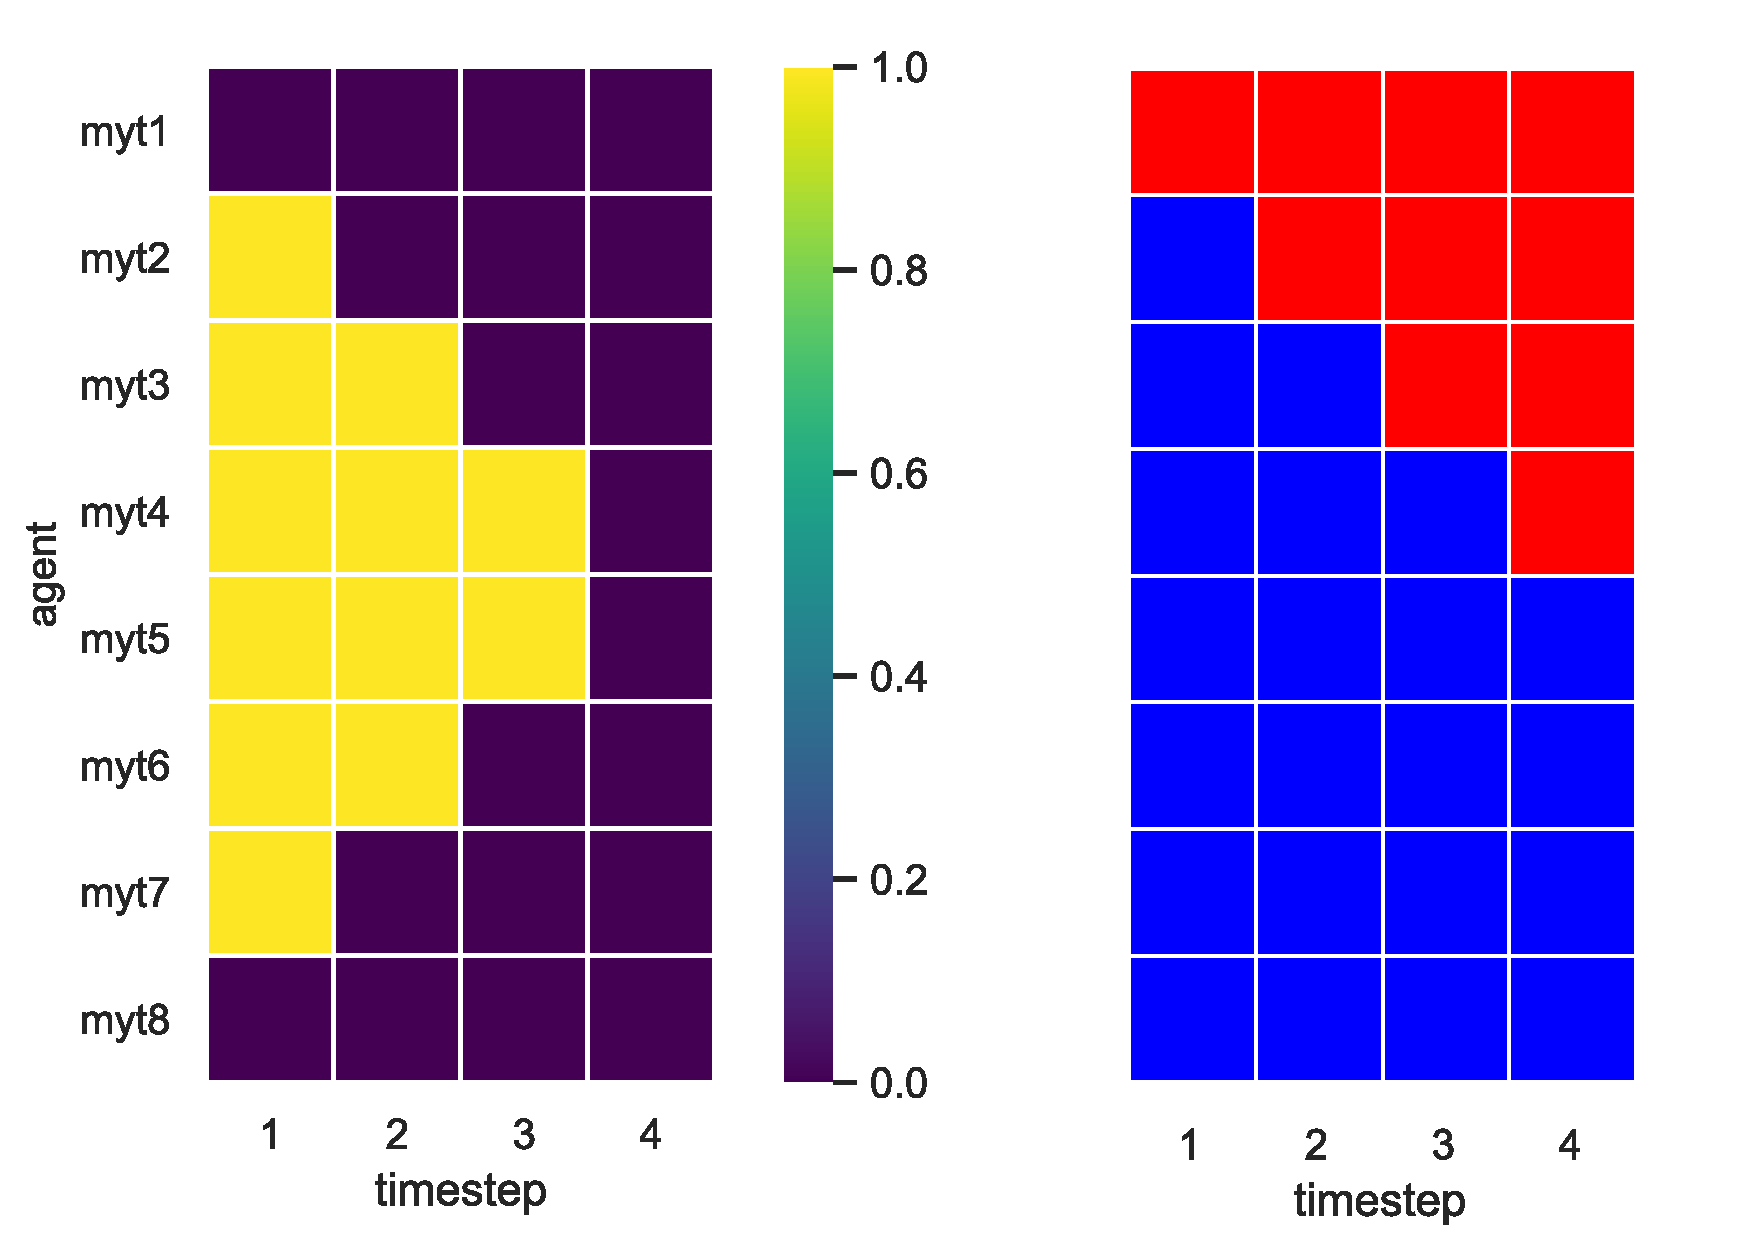
\includegraphics[width=.55\textwidth]{contents/images/net-v6/learned-0}
		\caption{Communication and colour decided using the learned controller.}
	\end{subfigure}
	\caption[Evaluation of the communication learned by 
	\texttt{net-v6}.]{Visualisation of the communication transmitted by each 
		robot over time and the colour decided by the controller learned from 
		\texttt{net-v6}.}	
	\label{fig:net-v6commcolour}
\end{figure}

Visualising in Figure \ref{fig:net-v6commcolour} the communication protocol 
inferred by the network and the one chosen by the manual controller, as well as 
the colour assumed by each robot, we immediately see a difference in both the 
figures.
This time it is possible to hypothesize the policy adopted by the network to send 
messages: as before, the extreme robots always send the same message but this 
time the central ones communicate a value interpreted as a reward. In detail, 
starting from the edges, the value 0 is transmitted, then, once the robot that 
follows or precedes receives this value in turn communicates 0, until all the agents 
have received the message and therefore have clear their positional order.
This type of reward acts in such a way as to colour as desired the following robot, 
for those in the first half, or the one that precedes, for those in the second, 
communicating 0 respectively when there is a red agent behind it or when in front 
there is a blue one. In this way the control is able to stabilise and achieve its goal.

In Figure \ref{fig:net-v6error} is presented the measure of the amount of wrong 
expected colours, on the y-axis, over time, averaged on all robots among all the 
simulation runs. 
As expected, the number of colours correctly predicted by the learned controller 
is lower than before, while the manual controller still has the same performance.  
\begin{figure}[!htb]
	\centering
	\includegraphics[width=.5\textwidth]{contents/images/net-v6/colours-errors-compressed}%
	\caption[Evaluation of \texttt{net-v6} amount of wrong expected 
	colours.]{Comparison of performance in terms of amount of wrong expected 
		colours obtained using the controller learned from \texttt{net-v6}.}
	\label{fig:net-v6error}
\end{figure}

We conclude the experiment on this task by presenting the results obtained using 
variable number of agents. In Figure \ref{fig:commlossnvart2} are summarised the 
performance in terms of loss, as before we used blue, orange and green lines to 
represent respectively average gaps of $8$\gls{cm}, $13$\gls{cm} and variable. 
As before we observe that in general the losses are increased respect the first 
experiment that use a smaller number of agents, since a higher amount of robots 
reduce the performance of the models, instead it is decreased respect the last 
experiment examined.
\begin{figure}[!htb]
	\centering
	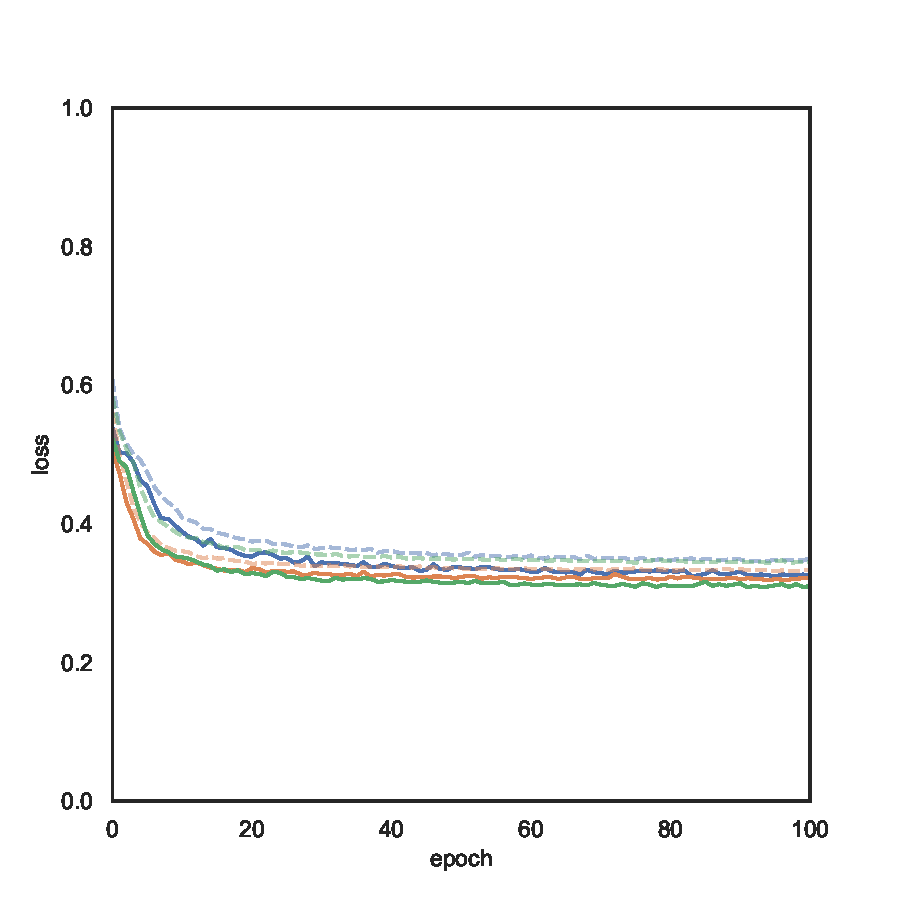
\includegraphics[width=.45\textwidth]{contents/images/task2/loss-communication-Nvar}
	\caption{Comparison of the losses of the models that use variable agents as the 
	gap varies.}
	\label{fig:commlossnvart2}
\end{figure}

\bigskip
\bigskip
From the \gls{roc} curve of the model in Figure \ref{fig:net-v9auc}  we observe 
that this time the \gls{auc} is a bit increased respect the previous experiment, 
going from $0.87$ up to $0.89$, but still worse than the first one.
%Instead the accuracy is decreased from a value of $73\%$ down to $71\%$ 
%respect the previous model examined.
\begin{figure}[!htb]
	\centering
	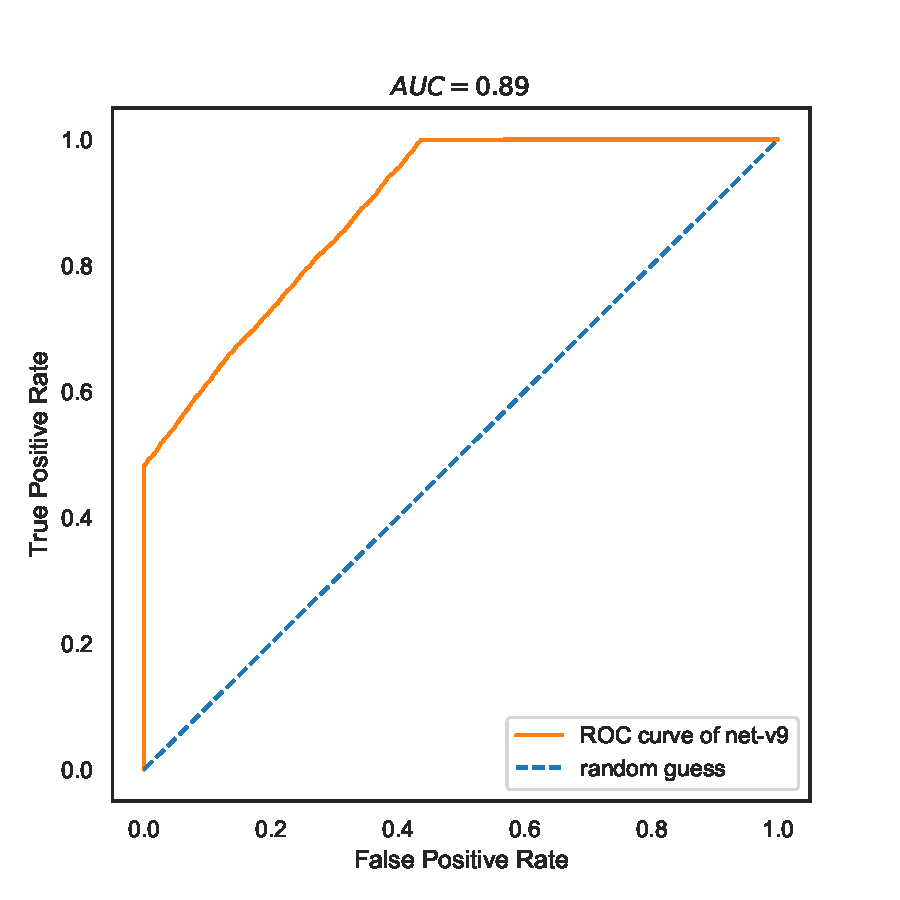
\includegraphics[width=.45\textwidth]{contents/images/net-v9/roc-net-v9(a)}%
	\caption[Evaluation of the \gls{roc} of \texttt{net-v9}.]{Visualisation of the 
		\gls{roc} curve of \texttt{net-v9}.}
	\label{fig:net-v9auc}
\end{figure}

This time we visualise in Figures \ref{fig:net-v9commcolour} and 
\ref{fig:net-v9commcolour2} two examples of communication protocol inferred 
by the network and the one chosen by the manual controller, as well as the colour 
assumed by each robot.
The first visualisation is obtained from a simulation with 10 agents. 
As before, the policy adopted by the network to send messages is very similar to 
the previous one. The robots at the edges start to transmit the value 0. Then, once 
the next robots receive the message in turn they communicates 0 or a value very 
close to it, until all the agents have received and sent the the message and have 
finally clear their positional order.
This time the manual and learned controllers achieve the goal in the same 
number of time steps.
\begin{figure}[!htb]
	\begin{subfigure}[h]{\textwidth}
		\centering
		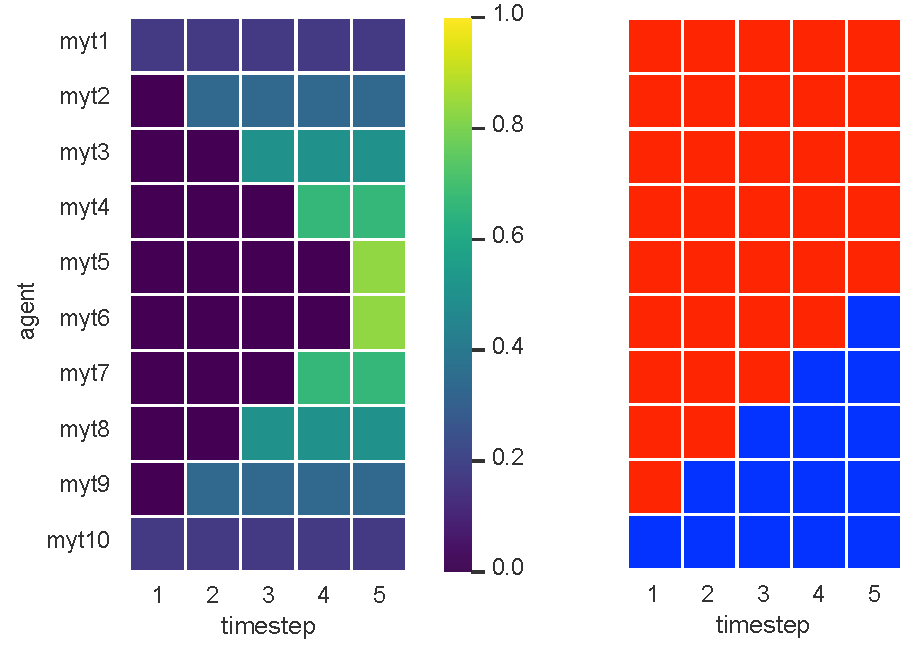
\includegraphics[width=.6\textwidth]{contents/images/net-v9/manual-0}
		\caption{Communication and colour decided using the manual controller.}
	\end{subfigure}
	\hspace*{\fill}%          % empty line absolutely necessary!
	\vspace*{8pt}%  
	\hspace*{\fill}%  
	\begin{subfigure}[h]{\textwidth}
		\centering			
		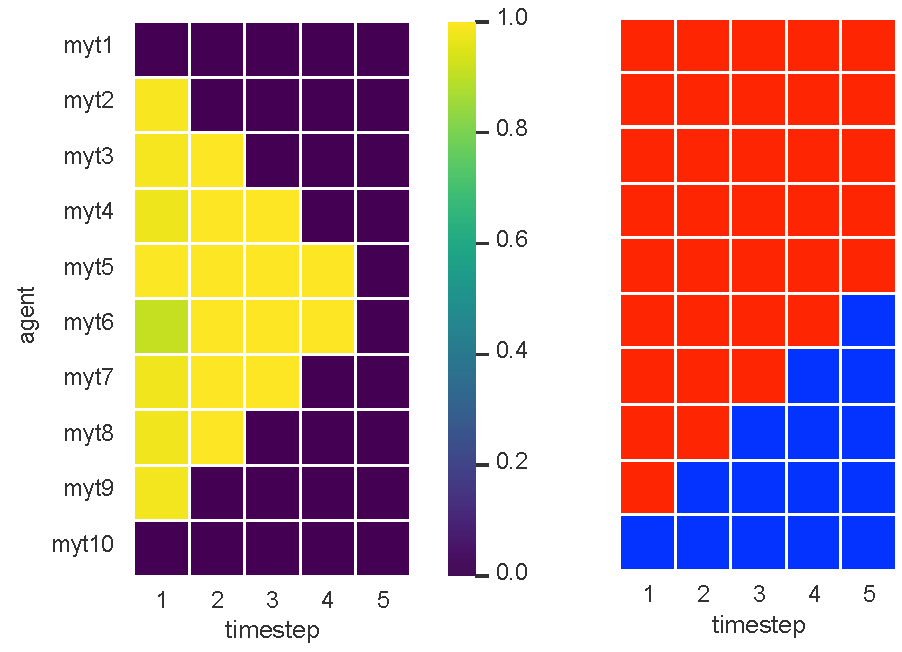
\includegraphics[width=.6\textwidth]{contents/images/net-v9/learned-0}
		\caption{Communication and colour decided using the learned controller.}
	\end{subfigure}
	\caption[Evaluation of the communication learned by 
	\texttt{net-v9}.]{Visualisation of the communication transmitted by each 
		robot over time and the colour decided by the controller learned from 
		\texttt{net-v9}.}	
	\label{fig:net-v9commcolour}
\end{figure}

\bigskip
The second visualisation is obtained from a simulation with 6 agents. 
The policy adopted by the network is the same as before, this time is even more 
efficient than the protocol used from the manual controller. In fact, in 2 time 
steps, one less then the other controller, the model is able to achieve the goal.
\begin{figure}[!htb]
	\begin{subfigure}[h]{\textwidth}
		\centering
		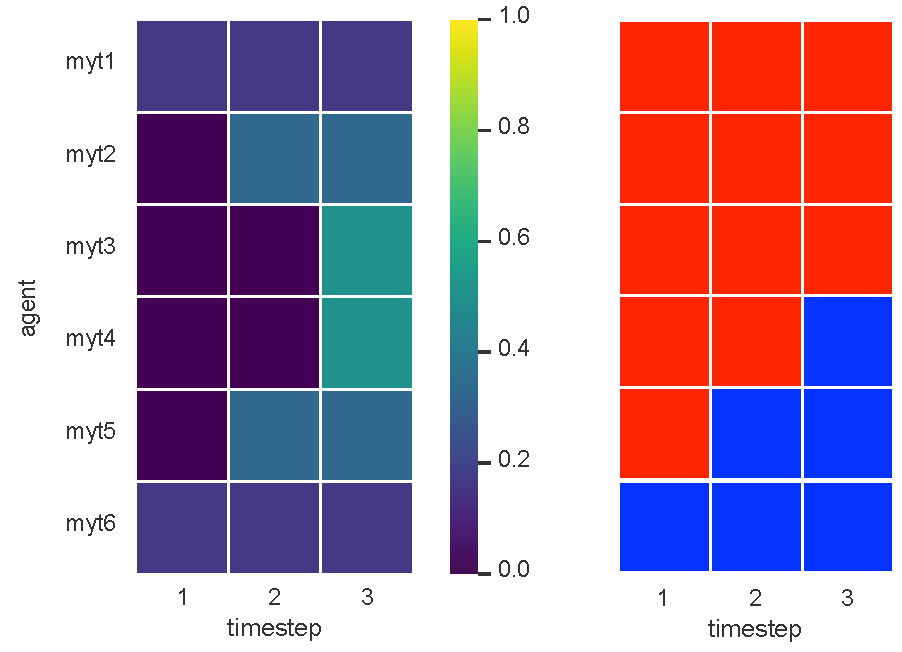
\includegraphics[width=.45\textwidth]{contents/images/net-v9/manual-1}
		\caption{Communication and colour decided using the manual controller.}
	\end{subfigure}
	\hspace*{\fill}%          % empty line absolutely necessary!
	\vspace*{8pt}%  
	\hspace*{\fill}%  
	\begin{subfigure}[h]{\textwidth}
		\centering			
		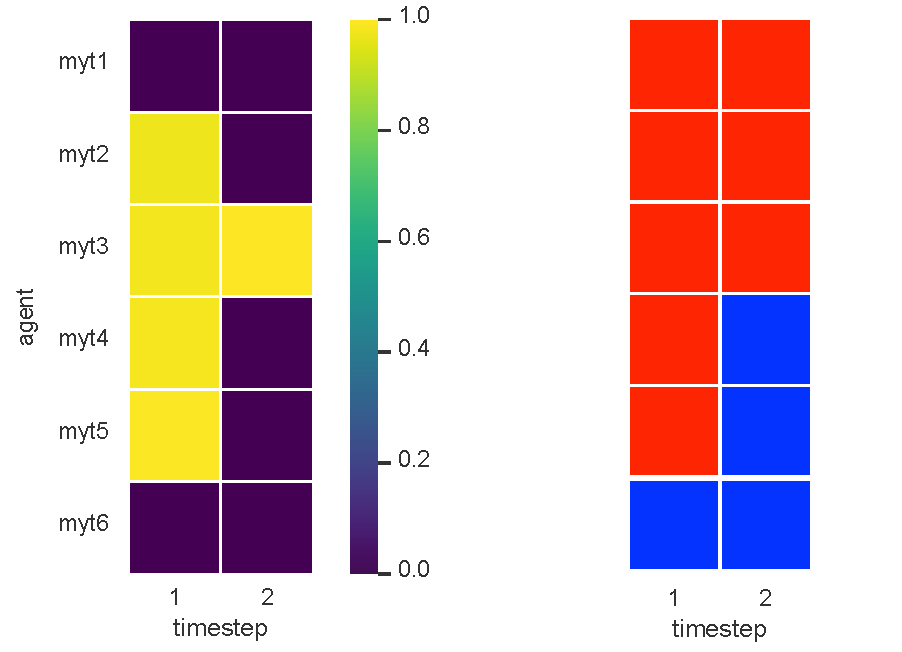
\includegraphics[width=.45\textwidth]{contents/images/net-v9/learned-1}
		\caption{Communication and colour decided using the learned controller.}
	\end{subfigure}
	\caption[Evaluation of the communication learned by 
	\texttt{net-v9}.]{Visualisation of the communication transmitted by each 
		robot over time and the colour decided by the controller learned from 
		\texttt{net-v9}.}	
	\label{fig:net-v9commcolour2}
\end{figure}

Finally, In Figure \ref{fig:net-v9error} is presented the measure of the amount of 
wrong expected colours, on the y-axis, over time, averaged on all robots among 
all the simulation runs. 
for this experiment the number of colours correctly predicted by the learned 
controller is a bit less than that obtained by the manual controller, and even if the 
variance for the model is higher the performance are acceptable.
\begin{figure}[!htb]
	\centering
	\includegraphics[width=.5\textwidth]{contents/images/net-v9/colours-errors-compressed}%
	\caption[Evaluation of \texttt{net-v9} amount of wrong expected 
	colours.]{Comparison of performance in terms of amount of wrong expected 
		colours obtained using the controller learned from \texttt{net-v9}.}
	\label{fig:net-v9error}
\end{figure}


\begin{figure}[!htb]
	\begin{center}
		\begin{subfigure}[h]{0.32\textwidth}
			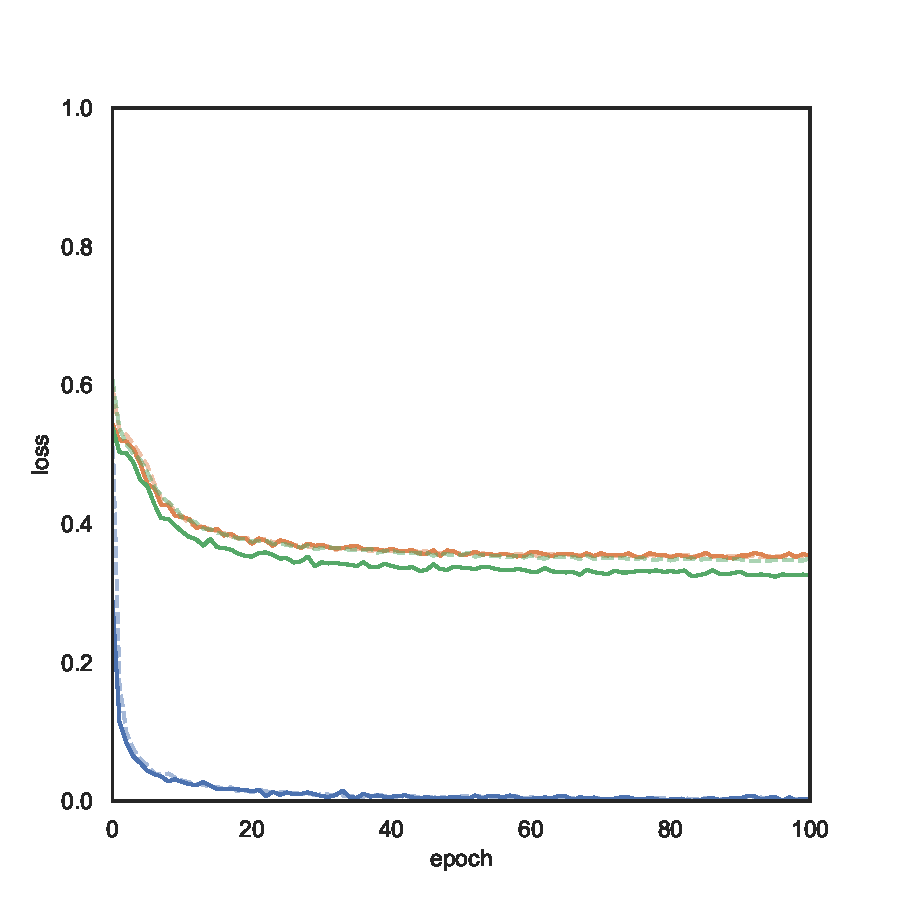
\includegraphics[width=\textwidth]{contents/images/task2/loss-communication-gap_8}%
			\caption{\texttt{avg\_gap} of $8$\gls{cm}.}
		\end{subfigure}
		\hfill
		\begin{subfigure}[h]{0.32\textwidth}
			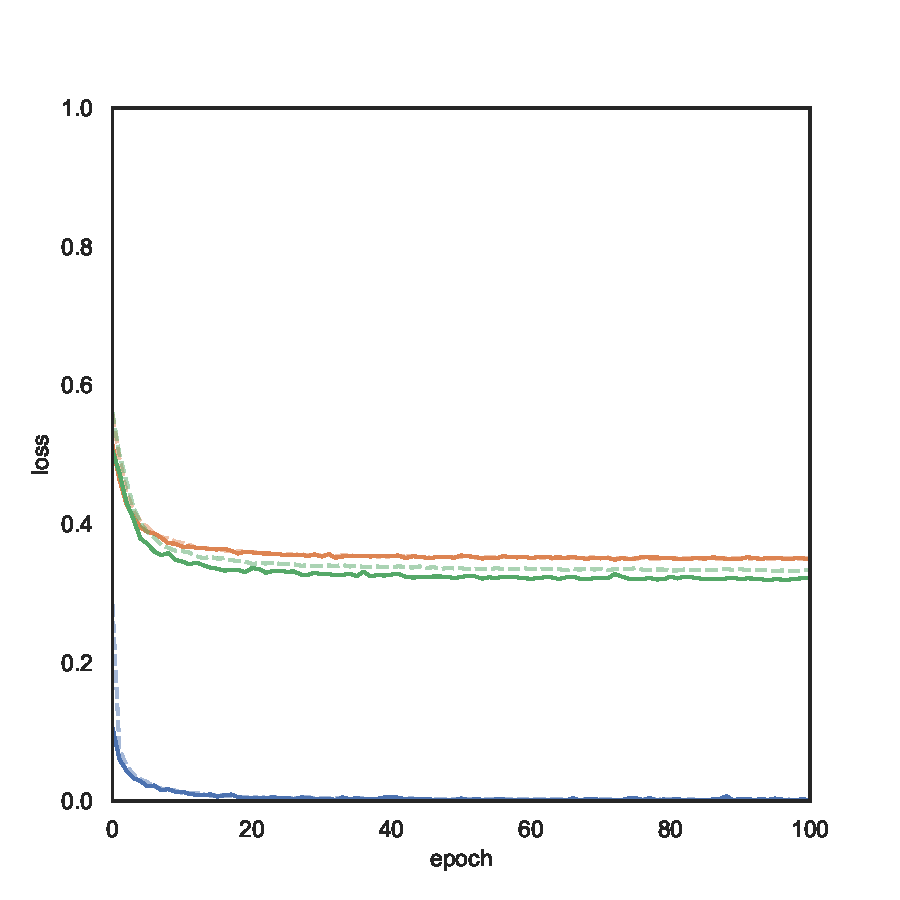
\includegraphics[width=\textwidth]{contents/images/task2/loss-communication-gap_20}%
			\caption{\texttt{avg\_gap} of $20$\gls{cm}.}
		\end{subfigure}
		\hfill
		\begin{subfigure}[h]{0.32\textwidth}
			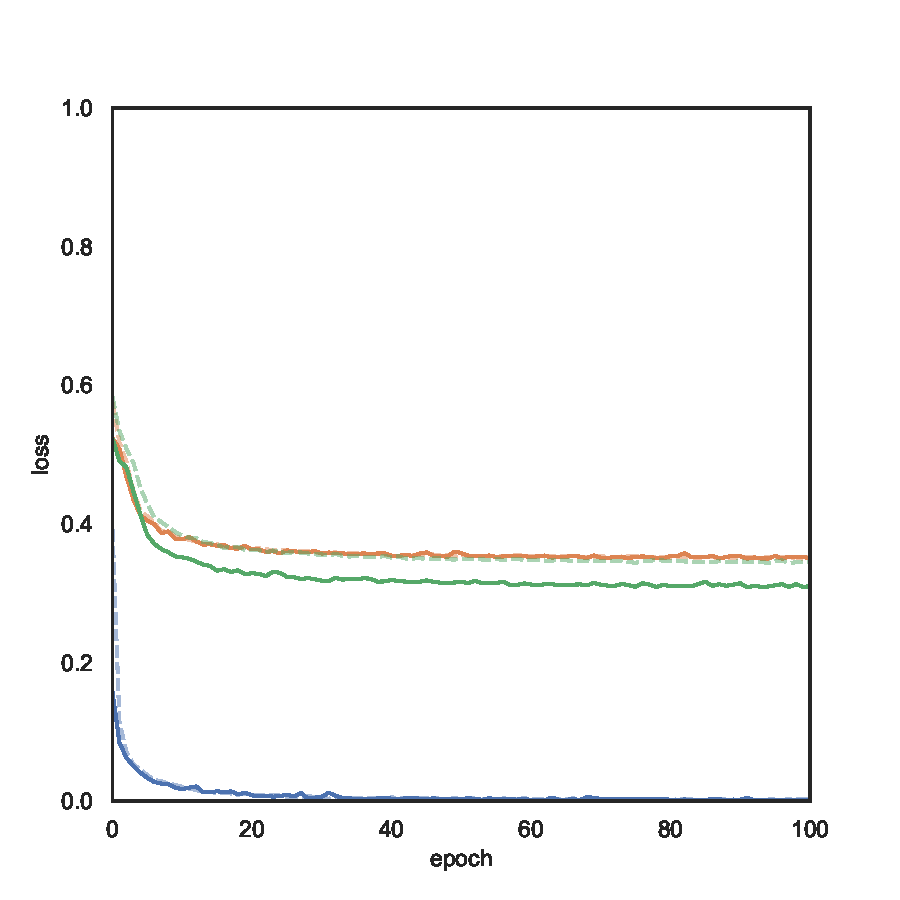
\includegraphics[width=\textwidth]{contents/images/task2/loss-communication-gap_var}
			\caption{\texttt{avg\_gap} variable.}
		\end{subfigure}
	\end{center}
	\vspace{-0.5cm}
	\caption[Losses summary of the second task (communication).]{Comparison of 
	the losses of the model trained with communication, by varying the number of 
	agents for the three gaps.}
	\label{fig:commlosst2}
\end{figure}
\subsubsection{Summary}
\label{subsubsec:summary1}

